\documentclass[a4paper]{tufte-handout}

\usepackage{iansnotes}

\title{Graph Isomorphism}
\author{iam.mcloughlin@gmit.ie}
\date{\today}
\begin{document}

\maketitle


\section{Basics}

    \begin{itemize}
        \item[Set:] $\{a, b, c\}$
        \item[Tuple:] $(a,a,a,b,c,d)$
        \item[Map:] $\{(a,d),(b,e),(c,d)\}$
    \end{itemize}



\section{Bijection}

    \begin{itemize}
        \item[Map] \( f : X \longleftrightarrow Y \)
        \item[Every $y$ in $Y$] is mapped to by exactly one $x$ in $X$
        \begin{marginfigure}
        \begin{adjustbox}{max width={\columnwidth}, center}
        \begin{tikzpicture}
          \begin{scope}[every node/.style={circle, fill=black, inner sep=1pt}]
            \node[label=left:\( a \)] (a1) at (0,2) {};
            \node[label=left:\( b \)] (a2) at (0,1) {};
            \node[label=left:\( c \)] (a3) at (0,0) {};

            \node[label=right:\( 1 \)] (b1) at (4,2) {};
            \node[label=right:\( 2 \)] (b2) at (4,1) {};
            \node[label=right:\( 3 \)] (b3) at (4,0) {};
          \end{scope}
          \begin{scope}[every fit/.style={ellipse, draw, inner sep=-2pt}]
            \node[draw, fit= (a1) (a2) (a3), minimum width=20mm] {} ;
            \node[draw, fit= (b1) (b2) (b3), minimum width=20mm] {} ;
          \end{scope}
          \path[->, >=latex, shorten <=2pt, shorten >=2pt]
            (a1) edge node[above] {\( f \)} (b1)
            (a2) edge node[above] {\( f \)} (b2)
            (a3) edge node[above] {\( f \)} (b3);  
        \end{tikzpicture} 
        \end{adjustbox}
        \end{marginfigure}
        \item[Means] map is reversible.
        \item[Counterexample:] $f(x) = x^2$.
    \end{itemize}


\section{Graph}
    \begin{itemize}
        \item[Graph:] $G = (V, E)$
        \item[Vertex:] element of $V = \{1,2,3,4\}$
        \item[Edge:] any 2-subset of $V$, e.g. $\{1, 2\}$
    \end{itemize}
    
\section{Example}
    \begin{itemize}
    \item[$V$:] $\{1,2,3,4\}$
    \begin{marginfigure}
    \begin{adjustbox}{max width={\columnwidth}, center}
    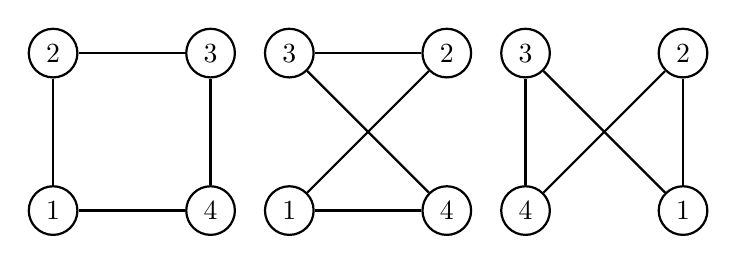
\begin{tikzpicture}
        \begin{scope}
            \begin{scope}[every node/.style={circle,thick,draw}]
              \node (a) at (0,0) {\( 1 \)};
              \node (b) at (0,2) {\( 2 \)};
              \node (c) at (2,2) {\( 3 \)};
              \node (d) at (2,0) {\( 4 \)};
            \end{scope}
            \begin{scope}[every edge/.style={draw=black,thick}]
                \path (a) edge (b)
                      (b) edge (c)
                      (c) edge (d)
                      (d) edge (a);
            \end{scope}
        \end{scope}
        \begin{scope}[xshift=30mm]
            \begin{scope}[every node/.style={circle,thick,draw}]
                \node (a) at (0,0) {\( 1 \)};
                \node (c) at (0,2) {\( 3 \)};
                \node (b) at (2,2) {\( 2 \)};
                \node (d) at (2,0) {\( 4 \)};
            \end{scope}
            \begin{scope}[every edge/.style={draw=black,thick}]
                \path (b) edge (c)
                      (c) edge (d)
                      (b) edge (a)
                      (d) edge (a);
            \end{scope}
        \end{scope}
        \begin{scope}[xshift=60mm]
            \begin{scope}[every node/.style={circle,thick,draw}]
                \node (a) at (0,0) {\( 4 \)};
                \node (b) at (0,2) {\( 3 \)};
                \node (c) at (2,2) {\( 2 \)};
                \node (d) at (2,0) {\( 1 \)};
            \end{scope}
            \begin{scope}[every edge/.style={draw=black,thick}]
                \path (a) edge (b)
                      (c) edge (d)
                      (c) edge (a)
                      (d) edge (b);
            \end{scope}
        \end{scope}
    \end{tikzpicture}
    \end{adjustbox}

    \end{marginfigure}
        \item[$E$:] $\{\{1,2\},\{1,4\},\{2,3\},\{3,4\}\}$
        \end{itemize}


\section{Isomorphism}

    \begin{itemize}
        \item[When] two graphs have the exact same structure.
        \item[$G_1 = (V_1,E_1)$] $\cong \  G_2=(V_2,E_2)$
        \item[$f:$] $V_1 \longleftrightarrow V_2$
        \item[$\{ f(x), f(y) \}$] $\in E_2 \  \Leftrightarrow \  \{ x, y \} \in  E_1$
        \begin{marginfigure}
        \begin{adjustbox}{max width={\columnwidth}, center}
        \begin{tikzpicture}
            \begin{scope}[every node/.style={circle, fill=black}]
                \node (a) at (1   , 1) {};
                \node (b) at (1   , 2) {};
                \node (c) at (0.33, 0) {};
                \node (d) at (1.66, 0) {};
            \end{scope}
            \begin{scope}[every edge/.style={draw=black, thick}]
                \path (a) edge (b)
                      (a) edge (c)
                      (a) edge (d)
                      (c) edge (d);
            \end{scope}
            \begin{scope}[every node/.style={circle, fill=black}]
                \node (1) at (6,2) {};
                \node (2) at (6,0) {};
                \node (3) at (8,2) {};
                \node (4) at (8,0) {};
            \end{scope}
            \begin{scope}[every edge/.style={draw=black, thick}]
                \path (1) edge (2)
                      (1) edge (3)
                      (1) edge (4)
                      (3) edge (4);
            \end{scope}
            \begin{scope}[every edge/.style={draw=gmitred, dashed, ->, >=latex}]
                \path (a) edge[bend left]  (1)
                      (b) edge[bend right] (2)
                      (c) edge[bend right] (3)
                      (d) edge[bend right] (4);
            \end{scope}
            \node at (1,-2) {\( G_1 \)};
            \node at (7,-2) {\( G_2 \)};
            \path (1.5,-2) edge[draw=gmitred, dashed, ->, >=latex] node[below] {\( f \)} (6.5,-2);
        \end{tikzpicture}
        \end{adjustbox}
        \end{marginfigure}
    \end{itemize}

\newpage 

\section{Exercise}
    \begin{figure}
    \begin{adjustbox}{max width={0.9\columnwidth}, center}
        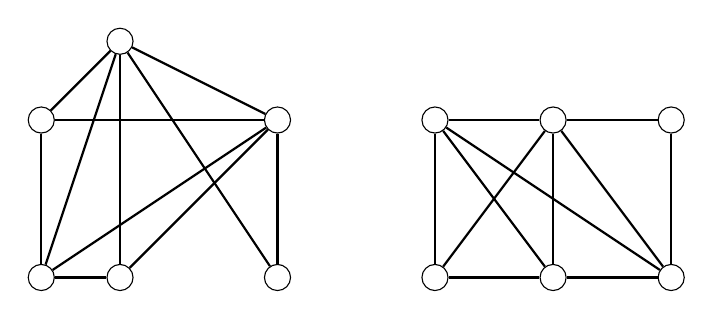
\begin{tikzpicture}
            \begin{scope}[every node/.style={circle,draw}]
                \node (a) at (0,0) {};
                \node (b) at (0,3) {};
                \node (c) at (2,0) {};
                \node (d) at (2,2) {};
                \node (e) at (-1,0) {};
                \node (f) at (-1,2) {};
            \end{scope}
            \begin{scope}[every edge/.style={draw=black,thick}]
                \path (a) edge (b);
                \path (a) edge (d);
                \path (a) edge (e);
                \path (b) edge (c);
                \path (b) edge (d);
                \path (b) edge (e);
                \path (b) edge (f);
                \path (c) edge (d);
                \path (d) edge (e);
                \path (d) edge (f);
                \path (e) edge (f);
            \end{scope}
            \begin{scope}[xshift=40mm]
                \begin{scope}[every node/.style={circle,draw}]
                    \node (a) at (0,0) {};
                    \node (b) at (0,2) {};
                    \node (c) at (1.5,0) {};
                    \node (d) at (1.5,2) {};
                    \node (e) at (3,0) {};
                    \node (f) at (3,2) {};
                \end{scope}
                \begin{scope}[every edge/.style={draw=black,thick}]
                    \path (a) edge (b);
                    \path (a) edge (c);
                    \path (c) edge (e);
                    \path (a) edge (d);
                    \path (b) edge (c);
                    \path (b) edge (d);
                    \path (b) edge (e);
                    \path (b) edge (d);
                    \path (d) edge (f);
                    \path (c) edge (d);
                    \path (d) edge (e);
                    \path (e) edge (f);
                \end{scope}
            \end{scope}
        \end{tikzpicture}
    \end{adjustbox}
    \caption{Are these isomorphic?}
    \end{figure}


\section{Adjacency Matrix}


    \begin{minipage}{0.3\columnwidth}
    \centering
    \begin{tabular}{ c|cccc } 
          & $1$ & $2$ & $3$ & $4$ \\
        \hline
        $1$ & $0$ & $1$ & $0$ & $1$ \\ 
        $2$ & $1$ & $0$ & $1$ & $0$ \\ 
        $3$ & $0$ & $1$ & $0$ & $1$ \\ 
        $4$ & $1$ & $0$ & $1$ & $0$ \\ 
    \end{tabular}
    \end{minipage}
        \begin{minipage}{0.3\columnwidth}
    \centering
    \begin{tabular}{ c|cccc } 
           & $1$ & $2$ & $3$ & $4$ \\
         \hline
         $1$ & $0$ & $0$ & $1$ & $1$ \\ 
         $2$ & $0$ & $0$ & $1$ & $1$ \\ 
         $3$ & $1$ & $1$ & $0$ & $0$ \\ 
         $4$ & $1$ & $1$ & $0$ & $0$ \\ 
    \end{tabular}
    \end{minipage}
    \begin{marginfigure}
    \begin{adjustbox}{max width={\columnwidth}, center}
    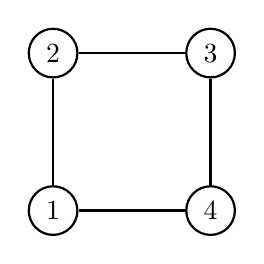
\begin{tikzpicture}
        \begin{scope}
            \begin{scope}[every node/.style={circle,thick,draw}]
              \node (a) at (0,0) {\( 1 \)};
              \node (b) at (0,2) {\( 2 \)};
              \node (c) at (2,2) {\( 3 \)};
              \node (d) at (2,0) {\( 4 \)};
            \end{scope}
            \begin{scope}[every edge/.style={draw=black,thick}]
                \path (a) edge (b)
                      (b) edge (c)
                      (c) edge (d)
                      (d) edge (a);
            \end{scope}
        \end{scope}
    \end{tikzpicture}
    \end{adjustbox}
    \end{marginfigure}

\section{Decision Problem}
    \begin{itemize}
        \item[Adjacency matrix 1:] $0101\ 1010\ 0101\ 1010$
        \item[Adjacency matrix 2:] $0011\ 0011\ 1100\ 1100$
        \item[String 1:] $101\ 10\ 1$\marginnote{Ignore the spaces - they are just for explanation.}
        \item[String 2:] $011\ 11\ 0$
        \item[Alphabet:] $\{0,1\}$
        \item[Language:] $L \subseteq A^*$
        \item[Graph Isomorphism Problem:] $L = \{ st | s \cong t \}$
        \item[Example:] $s_1 s_2 = 101 10 1 011 11 0 \in L $
    \end{itemize}


\end{document}
